\chapter{Joint Distributions}

The previous chapter studied one variable at a time, culminating in the normal
distribution. But most experiments produce several random quantities
simultaneously: height and weight, temperature across consecutive days, or blood
pressure and risk of disease.

To describe these relationships, we need a \emph{joint distribution} that
assigns probabilities to pairs $(X,Y)$ rather than to each variable in isolation.
We begin with discrete joint mass functions, move to continuous joint densities,
and see how marginals, conditioning, and independence arise naturally from the
joint picture.

\section{Two Dials at Once: The Joint PMF}
\label{ch13:joint-pmf}

Let us begin where intuition is safest: with discrete random variables, where a
probability distribution is just a list of outcomes and their probabilities.

\begin{intuitionbox}
Think of two random variables $X$ and $Y$ as two dials read off the \emph{same}
experiment. One spin of the experiment produces one reading on each dial, i.e.\
one pair $(x,y)$. The joint distribution is nothing more than the answer to:
``how often does each \emph{pair} of readings occur?'' If you have ever made a
two-way table -- rows for one category, columns for another, counts in the cells
-- you have already met a joint distribution.
\end{intuitionbox}

\begin{definition}[Joint PMF]
\label{ch13:def-joint-pmf}
Let $X$ and $Y$ be discrete random variables defined on the same sample space.
Their \emph{joint probability mass function} (joint PMF) is
\[
  p_{X,Y}(x,y) \;=\; \P(X = x,\ Y = y),
\]
where the comma means ``and'': the event that $X=x$ \emph{and} $Y=y$
simultaneously. (Recall that a probability mass function is simply a bookkeeping
rule that assigns a specific probability mass to each discrete outcome, like dots
of weight on a number line; a \emph{joint} PMF extends that bookkeeping to
pairs, placing a mass at each grid coordinate $(x,y)$ in the plane.)
A valid joint PMF satisfies $p_{X,Y}(x,y)\ge 0$ for all $(x,y)$ and
\[
  \sum_{x}\sum_{y} p_{X,Y}(x,y) \;=\; 1 .
\]
\end{definition}

The essential geometric shift in this chapter is to stop thinking of
$x$ and $y$ as separate axes processed in turn, and to start seeing the
\emph{pair} $(x,y)$ as the fundamental location in the plane. The joint PMF lives on the grid of all
possible pairs.

\begin{example}[A weather two-way table]
\label{ch13:ex-weather}
A meteorologist records two things each morning: $X$, whether it is cloudy
($X=1$) or clear ($X=0$); and $Y$, whether it rains that day ($Y=1$) or not
($Y=0$). Over many mornings she estimates the joint PMF in
Table~\ref{ch13:tab-weather}.

\begin{table}[H]
\centering
\begin{tabular}{c|cc|c}
 & $Y=0$ (dry) & $Y=1$ (rain) & row total \\
\hline
$X=0$ (clear)  & $0.55$ & $0.05$ & $0.60$ \\
$X=1$ (cloudy) & $0.15$ & $0.25$ & $0.40$ \\
\hline
col.\ total    & $0.70$ & $0.30$ & $1.00$ \\
\end{tabular}
\caption{Joint PMF of cloud cover $X$ and rain $Y$. The four interior cells are
$p_{X,Y}(x,y)$; the margins (literally the edges of the table) are the marginal
PMFs.}
\label{ch13:tab-weather}
\end{table}

The four interior numbers are the whole joint distribution. They sum to $1$.
Notice $p_{X,Y}(1,1)=0.25$: a cloudy, rainy day happens about a quarter of the
time. And $p_{X,Y}(0,1)=0.05$: rain out of a clear sky is rare. The table
already encodes a relationship -- rain clusters with clouds -- and our whole job
is to learn how to read that relationship off precisely.

\begin{recoverybox}
\textbf{Pause and think:} What is the probability that it either rains or is cloudy?
Looking at Table~\ref{ch13:tab-weather}, we sum the three matching cells:
$\P(X=1 \text{ or } Y=1) = p_{X,Y}(0,1) + p_{X,Y}(1,0) + p_{X,Y}(1,1) = 0.05 + 0.15 + 0.25 = 0.45$.
Equivalently, subtract the only excluded outcome (a dry, clear day):
$1 - p_{X,Y}(0,0) = 1 - 0.55 = 0.45$. Every probability question about $(X,Y)$
comes down to selecting the right cells and adding.
\end{recoverybox}
\end{example}

\begin{happeningbox}
A joint PMF is not two distributions glued together; it is \emph{one}
distribution over pairs. The reason this matters: knowing how $X$ behaves alone
and how $Y$ behaves alone is generally \emph{not enough} to reconstruct the
table. In Table~\ref{ch13:tab-weather} the row totals (how clouds behave) and
column totals (how rain behaves) are fixed, but you could rearrange the four
interior cells, keeping those totals, and get a completely different
relationship. The interior holds information the margins cannot see. That extra
information -- the \emph{dependence} -- gives joint distributions their
depth and character.
\end{happeningbox}

\subsection{Reading probabilities of events off the joint PMF}

Once you have the joint PMF, the probability of \emph{any} event described in
terms of $X$ and $Y$ is just a sum over the matching cells. Want
$\P(X \le Y)$? Sum $p_{X,Y}(x,y)$ over all pairs with $x\le y$. Want
$\P(X+Y = 1)$? Sum over the cells on the anti-diagonal. The joint PMF is a
complete description: every probabilistic question about the pair reduces to
adding up the right cells.

\begin{example}[Two dice, sum and max]
\label{ch13:ex-twodice}
Roll two fair dice. Let $X$ be the value on the first die and $Y$ the value on
the second. Because the dice are physically separate and fair, every pair
$(x,y)$ with $x,y\in\{1,\dots,6\}$ is equally likely, so
\[
  p_{X,Y}(x,y) = \tfrac{1}{36}, \qquad x,y \in \{1,\dots,6\}.
\]
This is the discrete uniform distribution on a $6\times 6$ grid. Now ask: what is
$\P(\max(X,Y) \le 4)$? The event $\max(X,Y)\le 4$ means \emph{both} dice are at
most $4$, i.e.\ all pairs in the $4\times4$ lower-left block: $16$ cells, each of
weight $1/36$, giving $16/36 = 4/9$. And $\P(X+Y=7)$? The anti-diagonal
$(1,6),(2,5),\dots,(6,1)$ has $6$ cells, so $6/36 = 1/6$. Every question is a
cell count divided by $36$.
\end{example}

Figure~\ref{ch13:fig-dicegrid} draws this joint PMF as what it literally is: a
grid of equal-probability points, with the two events above shaded. Reading a
probability is reading off how many dots fall in the shaded set.

\begin{figure}[H]
\centering
\begin{tikzpicture}[scale=0.72]
  % grid lines
  \draw[gray!40] (0.5,0.5) grid (6.5,6.5);
  % shade the max<=4 block
  \fill[sourceblue!18] (0.5,0.5) rectangle (4.5,4.5);
  % anti-diagonal x+y=7
  \foreach \x/\y in {1/6,2/5,3/4,4/3,5/2,6/1}{%
    \fill[quotientorange!30] (\x-0.5,\y-0.5) rectangle (\x+0.5,\y+0.5);}
  \draw[gray!40] (0.5,0.5) grid (6.5,6.5);
  % dots
  \foreach \x in {1,...,6}{\foreach \y in {1,...,6}{%
    \fill[distblue] (\x,\y) circle (2pt);}}
  % axis labels
  \foreach \t in {1,...,6}{%
    \node[font=\scriptsize] at (\t,0.1) {$\t$};
    \node[font=\scriptsize] at (0.1,\t) {$\t$};}
  \node[font=\small] at (3.5,-0.4) {first die $X$};
  \node[font=\small,rotate=90] at (-0.4,3.5) {second die $Y$};
  \node[font=\scriptsize\bfseries,sourceblue!70!black] at (2.5,2.5) {$\max\le 4$};
  \node[font=\scriptsize\bfseries,quotientorange!90!black,fill=white,inner sep=1.5pt,rounded corners=1pt] at (5.2,2.8) {$X+Y=7$};
\end{tikzpicture}
\caption{The joint PMF of two fair dice: $36$ equally likely points, each of
weight $1/36$. Blue block: $\max(X,Y)\le 4$ ($16$ points, probability $4/9$).
Orange anti-diagonal: $X+Y=7$ ($6$ points, probability $1/6$). For a discrete
joint distribution, a probability is just a weighted dot count.}
\label{ch13:fig-dicegrid}
\end{figure}

\section{Marginals: Collapsing the Table}
\label{ch13:marginals}

Suppose you have the joint PMF but you only care about $X$. You want
$p_X(x) = \P(X=x)$, ignoring $Y$ entirely. How do you get it?

\begin{intuitionbox}
``$X=x$'' happens whenever $X=x$ \emph{and} $Y$ takes \emph{some} value -- any
value at all. So to find how often $X=x$, you sweep across every possible $y$ and
add up the probabilities. On the two-way table this is exactly summing along a
row (or column). That is why these are called \emph{marginal} distributions:
historically you wrote the row and column sums in the \emph{margins} of the
table.
\end{intuitionbox}

\begin{definition}[Marginal PMFs]
\label{ch13:def-marginal-pmf}
From the joint PMF $p_{X,Y}$, the \emph{marginal PMFs} of $X$ and of $Y$ are
\[
  p_X(x) = \sum_{y} p_{X,Y}(x,y), \qquad
  p_Y(y) = \sum_{x} p_{X,Y}(x,y).
\]
\end{definition}

\begin{whybox}
Why does summing out $Y$ give the right answer for $X$? Because the events
$\{X=x, Y=y\}$, as $y$ ranges over all values, are \emph{disjoint} (you cannot
have two different $y$ readings on one trial) and \emph{exhaustive} of the event
$\{X=x\}$ (some $y$ always occurs). By the addition rule for disjoint events,
\[
  \P(X=x) = \P\!\Big(\bigcup_y \{X=x, Y=y\}\Big)
          = \sum_y \P(X=x, Y=y).
\]
This is the law of total probability applied to the partition of $\{X=x\}$ by the
value of $Y$. Nothing more mysterious is happening than ``slice the event into
non-overlapping pieces and add the pieces.''
\end{whybox}

In Table~\ref{ch13:tab-weather}, the marginal of $X$ is the column of row totals,
$p_X(0)=0.60,\ p_X(1)=0.40$; the marginal of $Y$ is the row of column totals,
$p_Y(0)=0.70,\ p_Y(1)=0.30$. So it is clear $60\%$ of the time and dry $70\%$ of
the time.

\begin{trapbox}
You can always go from the joint to the marginals (just add along rows/columns).
You can \emph{almost never} go the other way. Given only $p_X$ and $p_Y$, there
are usually many joint PMFs consistent with them. Marginals throw away the
relationship; collapsing the table is a one-way street. Whenever someone hands
you ``the distribution of $X$'' and ``the distribution of $Y$'' and asks about
both together, your first question must be: \emph{what is their joint behavior?}
\end{trapbox}

\section{Conditionals: Zooming Into One Row}
\label{ch13:conditionals}

Marginals forget about $Y$. Conditionals do the opposite: they \emph{fix} a value
of one variable and ask how the other is distributed in that slice of the world.

\begin{intuitionbox}
Suppose you walk outside and see that it is cloudy ($X=1$). You have learned
something. Among cloudy days, how often does it rain? You are no longer looking
at the whole table -- only at the cloudy row. But that row's entries
($0.15$ and $0.25$) sum to $0.40$, not $1$. To turn a row of a joint table into a
genuine probability distribution, you must \emph{renormalize}: divide each entry
by the row total ($0.40$) so the conditional probabilities sum to $1$.
(Renormalizing is just the rescaling step that forces any slice of relative weights
to behave like proper probabilities adding up to $100\%$.)
\end{intuitionbox}

\begin{definition}[Conditional PMF]
\label{ch13:def-cond-pmf}
For any $x$ with $p_X(x) > 0$, the \emph{conditional PMF} of $Y$ given $X=x$ is
\[
  p_{Y\given X}(y \given x)
  \;=\; \P(Y=y \given X=x)
  \;=\; \frac{p_{X,Y}(x,y)}{p_X(x)}.
\]
For each fixed $x$ this is a valid PMF in $y$: it is nonnegative and, summing
over $y$, the numerator sums to $p_X(x)$, which cancels the denominator to give
$1$.
\end{definition}

This is just the ordinary definition of conditional probability,
$\P(A\given B)=\P(A\cap B)/\P(B)$, with $A=\{Y=y\}$ and $B=\{X=x\}$. The
denominator $p_X(x)$ is exactly the marginal we computed by summing the row --
which is why marginals and conditionals are two sides of one coin.

\begin{example}[Rain given clouds]
\label{ch13:ex-rain-given-cloud}
From Table~\ref{ch13:tab-weather}, given a cloudy day ($X=1$, row total $0.40$):
\[
  p_{Y\given X}(1 \given 1) = \frac{0.25}{0.40} = 0.625,
  \qquad
  p_{Y\given X}(0 \given 1) = \frac{0.15}{0.40} = 0.375.
\]
So once you know it is cloudy, the rain probability jumps to $62.5\%$ -- far
above the unconditional $30\%$. Given a clear day ($X=0$, row total $0.60$):
\[
  p_{Y\given X}(1 \given 0) = \frac{0.05}{0.60} \approx 0.083 .
\]
Clouds raise the rain probability from $8.3\%$ to $62.5\%$. The variables clearly
inform each other; that is dependence, made quantitative.

\textbf{Pause and think:} If rain and clouds were completely unrelated, what would
$p_{Y\given X}(1\given 1)$ have been? It would have simply equaled the unconditional
probability of rain, $p_Y(1) = 0.30$. The leap from $0.30$ to $0.625$ measures
precisely how much the cloudy sky shifts our confidence.
\end{example}

Figure~\ref{ch13:fig-condbars} contrasts the marginal of $Y$ with the two
conditional distributions. Conditioning rebuilds the bars: a clear sky pushes
almost all the mass onto ``dry,'' a cloudy sky shifts the balance toward ``rain.''
If $X$ and $Y$ were independent, all three panels would be identical.

\begin{figure}[H]
\centering
\begin{tikzpicture}
\begin{axis}[
  ybar, bar width=12pt,
  width=12cm, height=5.2cm,
  ymin=0, ymax=1,
  ylabel={probability},
  symbolic x coords={dry,rain},
  xtick=data,
  enlarge x limits=0.5,
  legend style={at={(0.5,1.02)},anchor=south,legend columns=-1,font=\scriptsize},
  area legend,
  nodes near coords, nodes near coords style={font=\tiny, /pgf/number format/fixed, /pgf/number format/precision=2},
]
\addplot[fill=gray!45] coordinates {(dry,0.70) (rain,0.30)};
\addplot[fill=sourceblue!55] coordinates {(dry,0.917) (rain,0.083)};
\addplot[fill=quotientorange!70] coordinates {(dry,0.375) (rain,0.625)};
\legend{marginal $p_Y$, given clear ($X{=}0$), given cloudy ($X{=}1$)}
\end{axis}
\end{tikzpicture}
\caption{The marginal distribution of rain (gray) versus the two conditional
distributions. Each set of bars sums to $1$: conditioning fixes a row of
Table~\ref{ch13:tab-weather} and renormalizes it. The bars move because the
variables are dependent.}
\label{ch13:fig-condbars}
\end{figure}

\begin{focusbox}
Three objects, one table:
\begin{itemize}
  \item \textbf{Joint} $p_{X,Y}(x,y)$: a single cell -- ``both at once.''
  \item \textbf{Marginal} $p_X(x)$: a row total -- ``one variable, forget the
        other.''
  \item \textbf{Conditional} $p_{Y\given X}(y\given x)$: a row \emph{rescaled to
        sum to one} -- ``the other variable, given this one is fixed.''
\end{itemize}
And the bridge that ties them is one identity, the \emph{chain rule}:
\[
  p_{X,Y}(x,y) = p_X(x)\, p_{Y\given X}(y\given x)
              = p_Y(y)\, p_{X\given Y}(x\given y).
\]
Joint $=$ marginal $\times$ conditional. Read it left to right and it builds the
joint from a margin and a slice; read it right to left and it is the definition of
the conditional. You will use this constantly.
\end{focusbox}

\section{Independence of Random Variables}
\label{ch13:independence}

We can now say precisely what it means for two random variables to have
\emph{nothing to do with each other}.

\begin{intuitionbox}
$X$ and $Y$ are independent if learning the value of one tells you \emph{nothing}
about the distribution of the other. Concretely: the conditional distribution of
$Y$ given $X=x$ does not depend on $x$ at all -- every row of the table, once
renormalized, looks identical. If knowing $X$ never changes your beliefs about
$Y$, the two carry no information about each other.
\end{intuitionbox}

\begin{definition}[Independence, discrete case]
\label{ch13:def-indep}
Discrete random variables $X$ and $Y$ are \emph{independent}, written
$X \indep Y$, if their joint PMF factors into the product of the marginals:
\[
  p_{X,Y}(x,y) = p_X(x)\, p_Y(y) \qquad \text{for every pair } (x,y).
\]
Equivalently, $p_{Y\given X}(y\given x) = p_Y(y)$ for all $x$ with $p_X(x)>0$:
the conditional equals the marginal, so conditioning on $X$ changes nothing.
\end{definition}

\begin{whybox}
Why is the product rule the right definition? Independence of \emph{events} means
$\P(A\cap B)=\P(A)\P(B)$. Random-variable independence demands this for
\emph{every} pair of events of the form $A=\{X=x\}$ and $B=\{Y=y\}$:
\[
  \P(X=x, Y=y) = \P(X=x)\,\P(Y=y) \quad\text{for all } x,y.
\]
That is exactly the factorization $p_{X,Y}=p_X p_Y$. And it is genuinely
stronger than independence of just one chosen pair of events -- it must hold
across the \emph{whole} grid. If even one cell fails to equal the product of its
margins, the variables are dependent.
\end{whybox}

\begin{example}[Two dice are independent; sum and max are not]
\label{ch13:ex-dice-indep}
For the two fair dice of Example~\ref{ch13:ex-twodice},
$p_{X,Y}(x,y)=1/36$ while $p_X(x)=p_Y(y)=1/6$, and indeed
$\tfrac{1}{6}\cdot\tfrac{1}{6}=\tfrac{1}{36}$. So $X \indep Y$: the two physical
dice know nothing about each other.

But now let $S=X+Y$ and $M=\max(X,Y)$. These are \emph{not} independent. Knowing
$S=2$ forces $M=1$ (only $(1,1)$ gives sum $2$), whereas knowing $S=12$ forces
$M=6$. Learning the sum sharply constrains the max, so $S\not\indep M$. The
moral: independence is a property of \emph{specific} variables, not of the
experiment. Functions built from independent variables are usually \emph{not}
independent of each other.
\end{example}

\begin{trapbox}
Independence requires the factorization at \emph{every} cell. In
Table~\ref{ch13:tab-weather}, $p_X(1)p_Y(1)=0.40\times0.30=0.12$, but the actual
joint cell is $p_{X,Y}(1,1)=0.25\ne 0.12$. One mismatch is enough: clouds and
rain are dependent. You never need to check all cells to \emph{disprove}
independence -- a single counterexample does it.
\end{trapbox}

\begin{historybox}
The instinct to multiply probabilities when trials ``do not interfere'' is as
old as the subject itself. In the 1500s, Girolamo Cardano tallied dice games by
multiplying single-die outcomes, and in their celebrated 1654 correspondence on
the division of stakes in interrupted gambling, Blaise Pascal and Pierre de
Fermat did the same. Yet neither had a formal concept of a random variable, let
alone a joint distribution. For over two centuries, mathematicians possessed only
discrete combinatorics and single-variable calculus. They were thoroughly stuck
whenever two continuous quantities were entangled without one strictly dictating
the other: how could one formulate a mathematical law for two variables that
wander together, such as a parent's height and their adult child's height?

In the late 19th century, Francis Galton wrestled with this very question while
studying heredity. Lacking modern probability spaces, Galton and Karl Pearson
debated whether this mutual leaning represented a mysterious biological force or
could be captured by the pure geometry of a two-dimensional bell-shaped surface.
Meanwhile, continuous probability was rocked by controversy: Joseph Bertrand's
1889 paradox demonstrated that asking for a ``random chord'' across a circle
produced three completely contradictory probabilities depending on which coordinate
system was declared uniform, casting doubt on whether continuous joint models
could ever rest on solid mathematical ground.

The resolution arrived in 1933 when Andrei Kolmogorov published his axiomatic
foundations of probability. Framing random variables as measurable functions on
a shared sample space and joint distributions as probability measures over
regions in $\R^n$, Kolmogorov converted intuitive notions of non-interference
into the checkable product equation $p_{X,Y} = p_X p_Y$ (or $f_{X,Y} = f_X f_Y$).
Using the Radon--Nikodym theorem (the tool from measure theory that defines the
ratio of two measures, playing the role of a derivative for areas and
volumes), he proved that conditioning on a single measure-zero slice like
$\{X=x\}$ was mathematically rigorous rather than an undefined division by zero.
This foundation unlocked modern statistical physics (tracking the joint
coordinates and velocities of billions of colliding gas molecules), multivariate
statistics, and generative artificial intelligence. What remains an active
frontier is the ``curse of dimensionality'': as the number of interacting
variables climbs into the hundreds or thousands, data points become infinitely
sparse across high-dimensional space, making joint densities impossible to
estimate directly without strong structural tools such as copulas, graphical
models, and deep neural networks.
\end{historybox}

\section{Crossing to the Continuum: Joint Densities}
\label{ch13:joint-pdf}

Now let $X$ and $Y$ be continuous -- say a person's height and weight, each able
to take any real value in a range. We can no longer ask $\P(X=x, Y=y)$, because
for a continuous variable any single value has probability zero, and so does any
single point in the plane. The fix is exactly the one-dimensional fix, lifted to
two dimensions: probability is no longer mass sitting on points, but
\emph{volume} sitting under a surface.

\begin{intuitionbox}
In one dimension, a density $f_X(x)$ is a curve, and $\P(a\le X\le b)$ is the
\emph{area} under the curve between $a$ and $b$. In two dimensions, a joint
density $f_{X,Y}(x,y)$ is a \emph{surface} floating above the plane, and the
probability that $(X,Y)$ lands in a region $R$ is the \emph{volume} of the solid
under the surface and above $R$. Height of the surface $=$ how densely probability
is packed near that point. Tall surface $=$ likely neighborhood; flat ground
$=$ unlikely.
\end{intuitionbox}

\begin{definition}[Joint PDF]
\label{ch13:def-joint-pdf}
A function $f_{X,Y}\colon \R^2 \to \R$ is a \emph{joint probability density
function} (joint PDF) of $(X,Y)$ if $f_{X,Y}(x,y)\ge 0$ everywhere,
\[
  \int_{-\infty}^{\infty}\!\!\int_{-\infty}^{\infty} f_{X,Y}(x,y)\,\dd x\,\dd y = 1,
\]
and for every (reasonable) region $R \subseteq \R^2$,
\[
  \P\big((X,Y)\in R\big) = \iint_{R} f_{X,Y}(x,y)\,\dd x\,\dd y .
\]
(A density function represents probability per unit area: its height at a point
can exceed $1$, but the volume standing under the surface over any patch $R$
equals the probability of the pair landing in $R$.)
\end{definition}

\begin{connectionbox}
This is the multivariable calculus of the double integral, now applied to probability.
The double integral computes volumes under surfaces, and here that volume represents
probability. The standard integration tools apply directly: setting up non-rectangular
limits, changing the order of integration via Fubini's theorem, or converting to polar
coordinates for circular regions.
\end{connectionbox}

\subsection{The surface picture}

A joint density is a smooth surface hovering over the coordinate plane.
Figure~\ref{ch13:fig-surface} shows the density of a pair of independent standard
normals -- the two-dimensional bell, a single smooth hill centered at the origin.
The probability of any region is how much ``dirt'' or volume sits over it.

\begin{figure}[H]
\centering
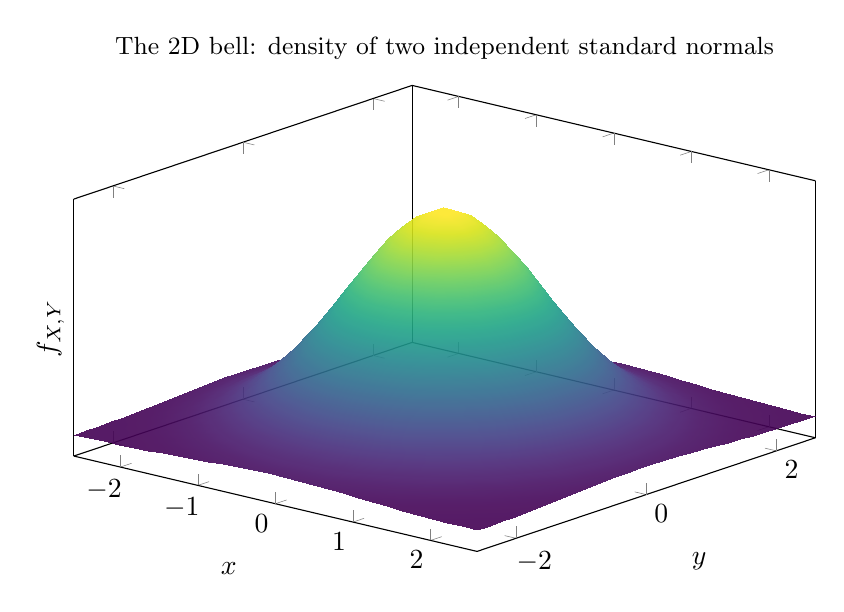
\begin{tikzpicture}
\begin{axis}[
  width=11cm, height=7.5cm,
  view={40}{30},
  domain=-2.6:2.6, y domain=-2.6:2.6,
  samples=28, samples y=28,
  xlabel={$x$}, ylabel={$y$}, zlabel={$f_{X,Y}$},
  ztick=\empty, colormap/viridis,
  title={The 2D bell: density of two independent standard normals},
  title style={font=\small},
]
\addplot3[surf, shader=interp, fill opacity=0.9]
  {0.15915*exp(-0.5*(x^2+y^2))};
\end{axis}
\end{tikzpicture}
\caption{The joint density $f_{X,Y}(x,y)=\frac{1}{2\pi}e^{-(x^2+y^2)/2}$ as a
surface. Probability is volume under this hill. It is tallest at the origin
(the most likely neighborhood) and decays smoothly in every direction.}
\label{ch13:fig-surface}
\end{figure}

Three-dimensional surfaces can be difficult to read quantitatively. The flat-map version is the
\emph{contour plot}: curves of constant density, like elevation lines on a topographic map. Figure~\ref{ch13:fig-contour} draws them. Concentric circles
mean the density depends only on distance from the center, and equal spacing of
the probability mass in every direction -- a signature, as we will see, of
independence plus rotational symmetry.

\begin{figure}[H]
\centering
\begin{tikzpicture}[scale=1.25]
  % Level curves of (1/2pi) e^{-(x^2+y^2)/2}=L are exact circles of
  % radius r = sqrt(-2 ln(2 pi L)). Inner rings = higher density.
  \fill[sourceblue!10] (0,0) circle (2.033); % L=0.02
  \fill[sourceblue!20] (0,0) circle (1.522); % L=0.05
  \fill[sourceblue!35] (0,0) circle (1.173); % L=0.08
  \fill[sourceblue!50] (0,0) circle (0.860); % L=0.11
  \fill[sourceblue!70] (0,0) circle (0.506); % L=0.14
  \draw[thick] (0,0) circle (2.033);
  \draw[thick] (0,0) circle (1.522);
  \draw[thick] (0,0) circle (1.173);
  \draw[thick] (0,0) circle (0.860);
  \draw[thick] (0,0) circle (0.506);

  % Axes spanning roughly [-2.8, 2.8]
  \draw[->] (-2.9,0)--(3.0,0) node[right]{$x$};
  \draw[->] (0,-2.9)--(0,3.0) node[above]{$y$};
  \foreach \t in {-1,1}{%
    \draw (\t,-0.05)--(\t,0.05) node[below=2pt,font=\scriptsize,fill=white,inner sep=1pt]{$\t$};
    \draw (-0.05,\t)--(0.05,\t) node[left=2pt,font=\scriptsize,fill=white,inner sep=1pt]{$\t$};
  }

  \fill[black] (0,0) circle (1.5pt);
  \node[font=\scriptsize\bfseries,fill=white,inner sep=1.5pt,rounded corners=1pt,anchor=east] at (-1.85,1.85) {peak $(0,0)$};
  \draw[->, >=stealth, black!75, thin] (-1.82,1.82) -- (-0.06,0.06);
  \node[font=\scriptsize,fill=white,inner sep=1.2pt,rounded corners=1pt] at (0.42,0.42) {$0.14$};
  \node[font=\scriptsize,fill=white,inner sep=1.2pt,rounded corners=1pt] at (1.18,1.18) {$0.05$};
  \node[font=\scriptsize,fill=white,inner sep=1.2pt,rounded corners=1pt] at (1.55,1.55) {$0.02$};
\end{tikzpicture}
\caption{Contours (level curves) of the 2D bell, drawn as the exact circles
$r=\sqrt{-2\ln(2\pi L)}$ for densities $L=0.02,0.05,0.08,0.11,0.14$. Each ring is
a set of points with equal density; the rings crowd together where the surface
falls off fastest. Reading a joint density as contours is the everyday tool of
data scientists looking at scatterplots of two variables.}
\label{ch13:fig-contour}
\end{figure}

\begin{happeningbox}
What is the height $f_{X,Y}(x,y)$, really? It is \emph{not} a probability -- it
can exceed $1$. It is a probability \emph{per unit area}, a density. The precise
statement is the small-rectangle approximation:
\[
  \P\big(x < X \le x+\dd x,\ y < Y \le y+\dd y\big)
  \;\approx\; f_{X,Y}(x,y)\,\dd x\,\dd y .
\]
Density times area equals (approximate) probability. This is the continuous echo
of ``$p_{X,Y}(x,y)$ is the probability of that cell'': a cell of the grid has
become an infinitesimal tile of the plane, and the density is the probability of
the tile divided by its area.
\end{happeningbox}

\section{Marginals and Conditionals in the Continuum}
\label{ch13:continuous-marg-cond}

Every idea from the discrete table survives the crossing, with sums replaced by
integrals. To get the marginal of $X$, you ``sum out'' $Y$ -- but summing out a
continuous variable means integrating it away.

\begin{definition}[Marginal PDFs]
\label{ch13:def-marginal-pdf}
\[
  f_X(x) = \int_{-\infty}^{\infty} f_{X,Y}(x,y)\,\dd y,
  \qquad
  f_Y(y) = \int_{-\infty}^{\infty} f_{X,Y}(x,y)\,\dd x.
\]
\end{definition}

\begin{intuitionbox}
Picture the surface again. To find $f_X(x)$ -- how dense $X$ is near a particular
$x$, ignoring $Y$ -- you stand at that $x$, slice the hill with a vertical plane
parallel to the $y$-axis, and \emph{add up the entire slice}: the integral
$\int f_{X,Y}(x,y)\,\dd y$ is the area of that cross-section. Tall fat slices mean
$x$ is a likely value of $X$. You are flattening the surface onto the $x$-axis by
letting all the $y$-probability rain straight down.
\end{intuitionbox}

\begin{definition}[Conditional PDF]
\label{ch13:def-cond-pdf}
For any $x$ with $f_X(x)>0$, the conditional density of $Y$ given $X=x$ is
\[
  f_{Y\given X}(y\given x) = \frac{f_{X,Y}(x,y)}{f_X(x)} .
\]
For fixed $x$ this is a valid density in $y$: it is the cross-section slice of the
surface at $x$, \emph{rescaled} (divided by its own area $f_X(x)$) so that it
integrates to $1$.
\end{definition}

Notice the perfect parallel. The conditional density is a vertical slice of the
joint surface, renormalized -- just as the discrete conditional was a row of the
table, renormalized. And conditioning on the measure-zero event $\{X=x\}$, which
looked illegal (you cannot divide by $\P(X=x)=0$), becomes legitimate the moment
you work with densities instead of probabilities: you divide by the
\emph{density} $f_X(x)$, which is generally positive (Figure~\ref{ch13:fig-slice-mountain}).

\begin{figure}[H]
\centering
\begin{tikzpicture}[scale=0.95]
  % Panel 1: Slicing the 3D surface
  \begin{scope}[shift={(0,0)}]
    \draw[draw=gray!30, fill=gray!3, rounded corners=4pt] (-2.9,-2.1) rectangle (2.9,3.8);
    \node[anchor=north, font=\small\bfseries, structurepurple!80!black] at (0,3.6) {1. Slicing Surface at $X = x_0$};

    % Coordinate axes (isometric projection)
    \draw[->, thick, gray!70] (0,0) -- (2.4,0) node[right, font=\scriptsize] {$y$};
    \draw[->, thick, gray!70] (0,0) -- (-1.6,-0.96) node[above left, font=\scriptsize] {$x$};
    \draw[->, thick, gray!70] (0,0) -- (0,2.6) node[above, font=\scriptsize] {$f_{X,Y}$};

    % Joint bell surface wireframe / contours
    \draw[gray!35, thin] (-1.6,-0.96) .. controls (0,0.8) .. (2.3,0);
    \draw[gray!35, thin] (-1.1,-0.66) .. controls (0,1.5) .. (1.6,0);

    % Cutting plane at x = x0 (x0 = 0.8 -> shift is (-0.6, -0.36))
    \coordinate (X0) at (-0.6, -0.36);
    \fill[quotientorange!12, draw=quotientorange!50, dashed, rounded corners=2pt]
      ($(X0)+(-1.6, -0.2)$) -- ($(X0)+(2.4, -0.2)$) -- ($(X0)+(2.4, 2.3)$) -- ($(X0)+(-1.6, 2.3)$) -- cycle;
    \node[font=\scriptsize\bfseries, quotientorange!80!black] at ($(X0)+(-0.8, 2.1)$) {Plane $X = x_0$};

    % Slice profile: cross-section curve at x = x0
    \fill[quotientorange!30]
      ($(X0)+(-1.5,0)$)
      \foreach \y/\z in {-1.5/0.05, -1.1/0.25, -0.7/0.85, -0.3/1.6, 0.0/1.85, 0.3/1.6, 0.7/0.85, 1.1/0.25, 1.5/0.05} {
        -- ($(X0)+(\y,\z)$)
      }
      -- ($(X0)+(1.5,0)$) -- cycle;

    \draw[densityred, very thick]
      ($(X0)+(-1.5,0.05)$)
      \foreach \y/\z in {-1.1/0.25, -0.7/0.85, -0.3/1.6, 0.0/1.85, 0.3/1.6, 0.7/0.85, 1.1/0.25, 1.5/0.05} {
        -- ($(X0)+(\y,\z)$)
      };
    \node[anchor=south west, font=\scriptsize\bfseries, densityred] at ($(X0)+(0.6, 1.2)$) {$z = f_{X,Y}(x_0, y)$};

    % Baseline on cutting plane
    \draw[thick, gray!80] ($(X0)+(-1.6,0)$) -- ($(X0)+(1.6,0)$);
    \fill[black] (X0) circle (1.5pt) node[below=2pt, font=\scriptsize] {$x_0$};

    % Annotation for slice area
    \node[align=center, font=\scriptsize, draw=quotientorange!80!black, fill=white, rounded corners=2pt, inner sep=2pt]
      at (0, -1.5) {Slice Area $= \displaystyle\int_{-\infty}^\infty f_{X,Y}(x_0, y)\,\dd y = f_X(x_0)$\\[1pt]\scriptsize (Marginal density of $X$ at $x_0$)};
  \end{scope}

  % Transmission arrow
  \draw[->, >=stealth, very thick, structurepurple] (3.3, 0.7) -- (5.0, 0.7)
    node[midway, above, font=\scriptsize\bfseries, align=center] {Renormalize\\[2pt]\tiny $\times \frac{1}{f_X(x_0)}$};

  % Panel 2: Rescaled 1D conditional density
  \begin{scope}[shift={(8.3,0)}]
    \draw[draw=gray!30, fill=gray!3, rounded corners=4pt] (-2.9,-2.1) rectangle (2.9,3.8);
    \node[anchor=north, font=\small\bfseries, sourceblue!80!black] at (0,3.6) {2. Conditional Density $f_{Y\mid X}$};

    % 2D axes
    \draw[->, thick, gray!70] (-2.2,0) -- (2.4,0) node[right, font=\scriptsize] {$y$};
    \draw[->, thick, gray!70] (0,0) -- (0,2.1);

    % Rescaled curve: total area = 1
    \fill[sourceblue!25]
      (-1.5,0)
      \foreach \y/\z in {-1.5/0.04, -1.1/0.22, -0.7/0.76, -0.3/1.43, 0.0/1.7, 0.3/1.43, 0.7/0.76, 1.1/0.22, 1.5/0.04} {
        -- (\y,\z)
      }
      -- (1.5,0) -- cycle;

    \draw[sourceblue!90!black, very thick]
      (-1.5,0.04)
      \foreach \y/\z in {-1.1/0.22, -0.7/0.76, -0.3/1.43, 0.0/1.7, 0.3/1.43, 0.7/0.76, 1.1/0.22, 1.5/0.04} {
        -- (\y,\z)
      };

    \node[above, font=\scriptsize\bfseries, sourceblue!90!black]
      at (0, 2.3) {$f_{Y\mid X}(y\mid x_0) = \frac{f_{X,Y}(x_0,y)}{f_X(x_0)}$};

    % Area annotation
    \node[align=center, font=\scriptsize, draw=sourceblue!80!black, fill=white, rounded corners=2pt, inner sep=2pt]
      at (0, -1.5) {Total Area $= \displaystyle\int_{-\infty}^\infty f_{Y\mid X}(y\mid x_0)\,\dd y = 1$\\[1pt]\scriptsize (A valid 1D probability density)};
  \end{scope}
\end{tikzpicture}
\caption{The geometry of continuous conditioning. Slicing the joint probability mountain at $X = x_0$ yields a 1D cross-sectional slice whose total area is the marginal density $f_X(x_0)$. Dividing the slice height by its own area renormalizes it into a legitimate 1D probability density $f_{Y\mid X}(y\mid x_0)$ integrating to $1$.}
\label{ch13:fig-slice-mountain}
\end{figure}

\begin{definition}[Independence, continuous case]
\label{ch13:def-indep-cont}
$X$ and $Y$ are independent if and only if their joint density factors:
\[
  f_{X,Y}(x,y) = f_X(x)\,f_Y(y) \quad\text{for all } (x,y),
\]
equivalently $f_{Y\given X}(y\given x) = f_Y(y)$. For the 2D bell,
$\frac{1}{2\pi}e^{-(x^2+y^2)/2} = \big(\tfrac{1}{\sqrt{2\pi}}e^{-x^2/2}\big)
\big(\tfrac{1}{\sqrt{2\pi}}e^{-y^2/2}\big)$: it splits into an $x$-part times a
$y$-part, so the two coordinates are independent standard normals. The exponent
splitting as a sum $x^2+y^2$ is exactly what makes the density a product.
\end{definition}

\begin{aestheticbox}
The contour plot carries a clean tell for independence. A joint
density factors into $g(x)h(y)$ exactly when the surface is a
``product surface'' -- the same $y$-profile at every $x$, up to vertical
scaling. For such a density the contours are symmetric about lines parallel to the
axes and never tilt. Dependence shows up as contours that \emph{tilt} or
\emph{bend}: an ellipse
slanted at $45^\circ$ says ``large $x$ tends to go with large $y$.'' You will
meet that tilted ellipse again in the next chapter under the name
\emph{correlation}. The geometry of the contours \emph{is} the relationship.
\end{aestheticbox}

\section{Uniform on a Region}
\label{ch13:uniform}

The cleanest continuous joint distribution is the one where the surface is
perfectly flat over some region and zero outside it: all of probability is spread
evenly, like jam over toast cut to the shape of $R$.

\begin{definition}[Uniform on a region]
\label{ch13:def-uniform}
$(X,Y)$ is \emph{uniform on a region} $R\subseteq\R^2$ of finite area
$\abs{R}$ if
\[
  f_{X,Y}(x,y) =
  \begin{cases}
    \dfrac{1}{\abs{R}}, & (x,y)\in R,\\[1.2ex]
    0, & \text{otherwise.}
  \end{cases}
\]
The constant $1/\abs{R}$ is forced: the volume under a flat sheet of height $h$
over a region of area $\abs{R}$ is $h\cdot\abs{R}$, and that must equal $1$.
\end{definition}

\begin{happeningbox}
When the density is constant, \emph{probability becomes geometry}. For any region
$A\subseteq R$,
\[
  \P\big((X,Y)\in A\big) = \iint_A \frac{1}{\abs{R}}\,\dd x\,\dd y
  = \frac{\abs{A}}{\abs{R}} = \frac{\text{area of } A}{\text{area of } R}.
\]
Computing a probability is computing an area ratio -- nothing more. This is the
modern, rigorous form of the old ``geometric probability'' that Buffon used in
1733 when he dropped needles on a floor of parallel lines and turned the chance
of a crossing into an integral involving $\pi$.
\end{happeningbox}

\begin{example}[Uniform on the unit square is independent; on the triangle is not]
\label{ch13:ex-uniform-square-triangle}
\textbf{Square.} Let $(X,Y)$ be uniform on the unit square
$R=[0,1]\times[0,1]$, so $f_{X,Y}=1$ on the square. The marginal of $X$ is
\[
  f_X(x) = \int_0^1 1\,\dd y = 1, \quad 0\le x\le 1,
\]
i.e.\ $X\sim\Unif(0,1)$, and by symmetry $Y\sim\Unif(0,1)$. Since
$f_{X,Y}(x,y) = 1 = f_X(x)f_Y(y)$, the coordinates are \emph{independent}.

\textbf{Triangle.} Now let $(X,Y)$ be uniform on the triangle
$T=\{(x,y): 0\le x\le 1,\ 0\le y\le x\}$ below the diagonal. Its area is
$\tfrac12$, so $f_{X,Y}=2$ on $T$ and $0$ elsewhere. The marginal of $X$ depends
on where you are, because the height of the triangle grows with $x$:
\[
  f_X(x) = \int_0^x 2\,\dd y = 2x, \quad 0\le x\le 1.
\]
So $X$ is \emph{not} uniform -- larger $x$ values are more likely, because there
is more triangle above them. And the conditional of $Y$ given $X=x$ is
\[
  f_{Y\given X}(y\given x) = \frac{2}{2x} = \frac1x, \quad 0\le y\le x,
\]
which is $\Unif(0,x)$: given $X=x$, $Y$ is uniform on the segment up to $x$. The
conditional distribution depends on $x$, so $X$ and $Y$ are \emph{dependent}.
Same flat density, totally different story -- because the \emph{shape of the
region} couples the variables. The region's geometry creates dependence even
though the density is constant.

\textbf{Pause and think:} From this triangular region, what is
$\P(Y > 0.5 \given X = 0.4)$? It is exactly zero, because along the vertical
slice $X=0.4$, the variable $Y$ cannot exceed $0.4$. The conditional support
changes with $X$, which is the geometric hallmark of dependence.
\end{example}

\begin{figure}[H]
\centering
\begin{tikzpicture}[scale=2.4]
% square
\begin{scope}
  \fill[sourceblue!18] (0,0) rectangle (1,1);
  \draw[thick] (0,0) rectangle (1,1);
  \draw[->] (-0.1,0)--(1.25,0) node[right]{$x$};
  \draw[->] (0,-0.1)--(0,1.25) node[above]{$y$};
  \node at (0.5,0.5) {$f=1$};
  \node at (0.5,-0.32) {\small square: $X\indep Y$};
\end{scope}
% triangle
\begin{scope}[xshift=2cm]
  \fill[quotientorange!22] (0,0)--(1,0)--(1,1)--cycle;
  \draw[thick] (0,0)--(1,0)--(1,1)--cycle;
  \draw[->] (-0.1,0)--(1.25,0) node[right]{$x$};
  \draw[->] (0,-0.1)--(0,1.25) node[above]{$y$};
  \draw[dashed,gray] (0,0)--(1,1) node[right]{\small $y=x$};
  \node at (0.72,0.28) {$f=2$};
  \node at (0.5,-0.32) {\small triangle: $X\not\indep Y$};
\end{scope}
\end{tikzpicture}
\caption{Two uniform distributions. Over the square the coordinates are
independent; over the triangle the very shape of the support ties them together.
Support shape alone can manufacture dependence.}
\label{ch13:fig-square-triangle}
\end{figure}

\begin{trapbox}
A fast independence test for \emph{any} joint density: $X$ and $Y$ can be
independent only if the support (the set where $f_{X,Y}>0$) is a \emph{rectangle}
(possibly infinite), aligned with the axes \emph{and} the density factors there.
If the region where the density lives is a triangle, a disk, or anything where the
allowed range of $y$ \emph{depends on} $x$, the variables are automatically
dependent -- because the conditional support changes with $x$. The triangle above
fails this test on sight, before you compute a single integral.
\end{trapbox}

\section{A Fully Worked Continuous Example}
\label{ch13:worked-continuous}

Let us run the entire machine on one nontrivial density, computing the
normalizing constant, both marginals, a conditional, and a region probability.

\begin{example}[A coupled density on the unit square]
\label{ch13:ex-coupled}
Let
\[
  f_{X,Y}(x,y) = c\,(x + y), \qquad 0\le x\le 1,\ 0\le y\le 1,
\]
and zero elsewhere. This surface tilts upward toward the corner $(1,1)$.

\textbf{Step 1: find $c$.} The total volume must be $1$:
\[
  \int_0^1\!\!\int_0^1 c(x+y)\,\dd x\,\dd y
  = c\int_0^1\!\Big[\tfrac{x^2}{2} + xy\Big]_{x=0}^{1}\dd y
  = c\int_0^1\!\Big(\tfrac12 + y\Big)\dd y
  = c\Big(\tfrac12+\tfrac12\Big) = c.
\]
So $c = 1$, and $f_{X,Y}(x,y) = x+y$ on the square.

\textbf{Step 2: marginal of $X$.} Integrate out $y$:
\[
  f_X(x) = \int_0^1 (x+y)\,\dd y
         = \Big[xy + \tfrac{y^2}{2}\Big]_{y=0}^{1}
         = x + \tfrac12, \qquad 0\le x\le 1.
\]
A quick sanity check: $\int_0^1 (x+\tfrac12)\,\dd x = \tfrac12+\tfrac12 = 1$.
Good -- it is a valid density. By the symmetry of $x+y$ in its two arguments,
$f_Y(y) = y + \tfrac12$ as well.

\textbf{Step 3: are they independent?} Test the factorization:
\[
  f_X(x)f_Y(y) = \big(x+\tfrac12\big)\big(y+\tfrac12\big)
  = xy + \tfrac{x}{2} + \tfrac{y}{2} + \tfrac14,
\]
which is \emph{not} equal to $x+y$. So $X$ and $Y$ are \emph{dependent}. (The
support is a nice square, so the rectangle test does not rule out independence --
but the density still fails to factor, and that settles it.)

\textbf{Step 4: a conditional.} Given $X = x$,
\[
  f_{Y\given X}(y\given x) = \frac{x+y}{x+\tfrac12}, \qquad 0\le y\le 1.
\]
For $x = 0$ this is $f_{Y\given X}(y\given 0) = \frac{y}{1/2} = 2y$, a density
that \emph{rises} with $y$ -- given $X=0$, larger $Y$ is favored. At the
opposite edge, $x = 1$, we get
$\frac{1+y}{3/2} = \tfrac23(1+y)$, which is much flatter. So the shape of $Y$'s
distribution genuinely shifts as $x$ changes; that shifting \emph{is} the
dependence, seen up close.

\textbf{Step 5: a region probability.} What is $\P(X+Y \le 1)$? Integrate the
density over the lower-left triangle $\{x\ge0,\,y\ge0,\,x+y\le1\}$, illustrated
in Figure~\ref{ch13:fig-region-triangle}:
\[
  \P(X+Y\le 1) = \int_0^1\!\!\int_0^{\,1-x}(x+y)\,\dd y\,\dd x.
\]

\begin{figure}[H]
\centering
\begin{tikzpicture}[scale=3.0]
  % Shaded region X + Y <= 1
  \fill[sourceblue!22] (0,0) -- (1,0) -- (0,1) -- cycle;

  % Unit square dashed border
  \draw[dashed, gray!60] (0,0) rectangle (1,1);

  % Axes
  \draw[->, thick, gray!70] (-0.1,0) -- (1.25,0) node[right, font=\small] {$x$};
  \draw[->, thick, gray!70] (0,-0.1) -- (0,1.25) node[above, font=\small] {$y$};

  % Boundary line x + y = 1
  \draw[thick, sourceblue!80!black] (0,1) -- (1,0) node[pos=0.68, above right=-2pt, font=\scriptsize] {$x+y=1$};

  % Vertical integration slice at x = 0.45
  \draw[very thick, densityred] (0.45, 0) -- (0.45, 0.55);
  \fill[densityred] (0.45, 0) circle (0.8pt) node[below=2pt, font=\scriptsize] {$x$};
  \fill[densityred] (0.45, 0.55) circle (0.8pt) node[above right=1pt, font=\scriptsize] {$(x, 1-x)$};

  % Inner integral direction arrow
  \draw[->, >=stealth, thick, densityred] (0.45, 0.12) -- (0.45, 0.43)
    node[midway, right=2pt, font=\tiny] {$\dd y$};

  % Region labels
  \node[font=\footnotesize\bfseries, sourceblue!80!black] at (0.16,0.18) {$X+Y \le 1$};
  \node[font=\footnotesize, gray!60] at (0.75,0.75) {$X+Y > 1$};

  % Axis ticks
  \draw (1,0.02) -- (1,-0.02) node[below=2pt, font=\scriptsize] {$1$};
  \draw (0.02,1) -- (-0.02,1) node[left=2pt, font=\scriptsize] {$1$};
  \node[below left=1pt, font=\scriptsize] at (0,0) {$0$};
\end{tikzpicture}
\caption{Setting up the double integral for $\P(X+Y\le 1)$ on the unit square.
For each fixed $x \in [0,1]$, the vertical slice enters the region at the bottom
boundary $y=0$ and exits at the line $y=1-x$. Integrating $f_{X,Y}(x,y)$ along this
slice yields $\int_0^{1-x}(x+y)\,\dd y$; summing all slices from $x=0$ to $x=1$ gives
the total probability $1/3$.}
\label{ch13:fig-region-triangle}
\end{figure}

The inner integral sums the vertical slice at $x$:
\[
  \int_0^{1-x}(x+y)\,\dd y
  = \Big[xy + \tfrac{y^2}{2}\Big]_0^{1-x}
  = x(1-x) + \tfrac{(1-x)^2}{2}.
\]
Expand: $x - x^2 + \tfrac12(1 - 2x + x^2) = \tfrac12 - \tfrac12 x^2$. Then
\[
  \P(X+Y\le1) = \int_0^1\Big(\tfrac12 - \tfrac12 x^2\Big)\dd x
  = \tfrac12 - \tfrac16 = \tfrac13.
\]
So the pair falls in the lower triangle a third of the time. (Sensible: the
density leans toward $(1,1)$, the \emph{upper} corner, so it should favor the
upper triangle $X+Y>1$, which gets the remaining $2/3$.)
\end{example}

\begin{labbox}
Try the twin computation yourself with $f_{X,Y}(x,y) = c\,x\,y$ on the unit
square. (a) Show $c=4$. (b) Find $f_X$ and $f_Y$. (c) Show that this one
\emph{does} factor, so here $X\indep Y$ -- a useful contrast with the $x+y$
example, where the same square support gave dependence. Multiplication factors;
addition does not.
\end{labbox}

\section{A Discrete Worked Example with Real Dependence}
\label{ch13:worked-discrete}

\begin{example}[Drawing without replacement]
\label{ch13:ex-without-replacement}
A box holds $3$ red and $2$ blue balls. Draw two balls \emph{without}
replacement. Let $X=1$ if the first ball is red (else $0$), and $Y=1$ if the
second is red. Because the first draw changes what is left, $X$ and $Y$ should be
dependent -- let us build the joint PMF and confirm.

By the chain rule, $p_{X,Y}(x,y) = p_X(x)\,p_{Y\given X}(y\given x)$. The first
draw: $p_X(1) = 3/5$, $p_X(0) = 2/5$. After a red first draw, $2$ red and $2$
blue remain, so $p_{Y\given X}(1\given 1) = 2/4$. After a blue first draw, $3$ red
and $1$ blue remain, so $p_{Y\given X}(1\given 0) = 3/4$. Multiplying:

\begin{table}[H]
\centering
\begin{tabular}{c|cc|c}
 & $Y=0$ & $Y=1$ & $p_X$ \\
\hline
$X=0$ & $\tfrac{2}{5}\cdot\tfrac14 = \tfrac{1}{10}$
      & $\tfrac{2}{5}\cdot\tfrac34 = \tfrac{3}{10}$ & $\tfrac{2}{5}$ \\[0.6ex]
$X=1$ & $\tfrac{3}{5}\cdot\tfrac24 = \tfrac{3}{10}$
      & $\tfrac{3}{5}\cdot\tfrac24 = \tfrac{3}{10}$ & $\tfrac{3}{5}$ \\[0.6ex]
\hline
$p_Y$ & $\tfrac{2}{5}$ & $\tfrac{3}{5}$ & $1$ \\
\end{tabular}
\caption{Joint PMF for two draws without replacement.}
\label{ch13:tab-without-replacement}
\end{table}

The four cells sum to $1$. Now read off the lessons.

\emph{The marginals are equal.} Summing the columns gives
$p_Y(1) = \tfrac{3}{10}+\tfrac{3}{10} = \tfrac{3}{5}$, the same as $p_X(1)$! The
second ball is red with probability $3/5$ too. This is the (initially surprising)
``symmetry of draws'': \emph{before you look}, the second draw is just as likely
to be red as the first. Marginally, $Y$ behaves exactly like $X$.

\emph{But they are dependent.} Check a cell: $p_{X,Y}(1,1) = 3/10$, while
$p_X(1)p_Y(1) = \tfrac35\cdot\tfrac35 = \tfrac{9}{25} = 0.36 \ne 0.30$. The
factorization fails, so $X\not\indep Y$. Equivalently, $p_{Y\given X}(1\given 1)
= \tfrac12$ but $p_{Y\given X}(1\given 0)=\tfrac34$: knowing the first ball
\emph{does} change the odds on the second. Identical marginals, genuine
dependence -- a clean reminder that marginals do not determine the joint.
\end{example}

\begin{paradoxbox}
\textbf{Two coins, the ``other child,'' and why the joint is everything.} A
family has two children; you learn ``at least one is a boy.'' What is the chance
both are boys? Let $X,Y$ be the sexes of the (ordered) children, each
independent and equally likely $\{B,G\}$, so the four pairs $BB,BG,GB,GG$ each
have probability $1/4$. ``At least one boy'' removes only $GG$, leaving
$\{BB,BG,GB\}$, of which one is $BB$:
\[
  \P(\text{both boys}\given \text{at least one boy}) = \frac{1/4}{3/4}
  = \frac13,
\]
not $1/2$. The trap is to reason about one child at a time; the resolution is to
reason on the \emph{joint} sample space of pairs and condition there. Now change
the information to ``the \emph{older} child is a boy'' -- this fixes $X=B$ and
leaves $\{BB, BG\}$, giving $1/2$. Same family, different conditioning event,
different answer. The paradox dissolves the instant you insist on conditioning
inside the joint distribution rather than juggling marginals. The joint
distribution is not a luxury; it is the only place these questions are
well-posed.
\end{paradoxbox}

\section{Beyond Two: Joint Distributions of Many Variables}
\label{ch13:many}

Everything generalizes to $n$ random variables. The joint PMF or PDF lives on
$n$-tuples, and marginals come from summing or integrating out all the variables
you do not want. The chain rule telescopes:
\[
  p(x_1,\dots,x_n) = p(x_1)\,p(x_2\given x_1)\,p(x_3\given x_1,x_2)\cdots
                     p(x_n\given x_1,\dots,x_{n-1}).
\]
And \emph{mutual independence} means the joint is the product of all the
marginals:
\[
  f(x_1,\dots,x_n) = f_1(x_1)\,f_2(x_2)\cdots f_n(x_n).
\]
The most important special case in all of statistics is a sequence of variables
that are \emph{independent and identically distributed} (i.i.d.): they share one
marginal $f$ and their joint is simply $\prod_i f(x_i)$. That single product is
the foundation of the laws of large numbers, the central limit theorem, and the
likelihood function of nearly every statistical model.

\begin{applicationbox}
\textbf{The likelihood function is a joint density read backwards.} In machine
learning and statistics you observe data $x_1,\dots,x_n$ and posit a model with
an unknown parameter $\theta$. If the data are i.i.d.\ from a density
$f(x;\theta)$, their \emph{joint} density is
\[
  L(\theta) = \prod_{i=1}^{n} f(x_i;\theta).
\]
Read as a function of the \emph{data} with $\theta$ fixed, this is an ordinary
joint density. Read as a function of $\theta$ with the data fixed, it is the
\emph{likelihood}, and the value of $\theta$ that maximizes it is the maximum
likelihood estimate -- standard for fitting models, from logistic regression
to neural networks (where the log-likelihood becomes the cross-entropy loss). The
product structure -- which is to say, the assumption of independence -- is what
turns a hairy joint object into a sum of log-terms you can differentiate. Whole
fields rest on the factorization $f=\prod f_i$.
\end{applicationbox}

\begin{connectionbox}
When all the variables are jointly normal, their joint density is governed by a
\emph{covariance matrix} $\Sigma$ -- a square table of numbers recording the
variance of each variable down the main diagonal and the pairwise associations
in the off-diagonal entries. The contours of the density are ellipses whose
principal axes align with the \emph{eigenvectors} of $\Sigma$ (the perpendicular
directions along which the probability cloud stretches most and least).
Independence corresponds to a diagonal $\Sigma$ (axis-aligned ellipses, like our
circular 2D bell); dependence tilts the ellipses. This is where probability
meets linear algebra directly: the geometry of a Gaussian cloud is the
spectral theorem in action (the linear algebra guarantee that every symmetric
matrix decomposes into perpendicular axes of stretch). We develop covariance in
the next chapter, and the multivariate normal in full later; the companion linear
algebra book's chapter on symmetric matrices and the spectral theorem is the
natural partner.
\end{connectionbox}

\section{Summary}
\label{ch13:summary}

\begin{recoverybox}
The core concepts of this chapter:
\begin{itemize}
  \item A \textbf{joint distribution} describes two (or more) random variables
        \emph{together}: a PMF $p_{X,Y}(x,y)$ on a grid (discrete), or a density
        $f_{X,Y}(x,y)$ as a surface with probability $=$ volume (continuous).
  \item \textbf{Marginals} come from collapsing the joint -- sum or integrate out
        the unwanted variable: $p_X(x)=\sum_y p_{X,Y}$,
        $f_X(x)=\int f_{X,Y}\,\dd y$. One-way street: joint $\to$ marginals,
        never back.
  \item \textbf{Conditionals} come from fixing one variable and renormalizing the
        slice: $p_{Y\given X}=p_{X,Y}/p_X$, $f_{Y\given X}=f_{X,Y}/f_X$. The
        bridge is the \textbf{chain rule}: joint $=$ marginal $\times$ conditional.
  \item \textbf{Independence} is the factorization
        $p_{X,Y}=p_X p_Y$ (resp.\ $f_{X,Y}=f_X f_Y$), equivalently
        ``conditional $=$ marginal.'' It must hold \emph{everywhere}; one
        mismatch breaks it. Non-rectangular support guarantees dependence.
  \item \textbf{Uniform on a region} turns probability into an area ratio:
        $\P((X,Y)\in A) = \abs{A}/\abs{R}$.
\end{itemize}
Hold onto the surface-and-contours picture; it is the mental image that makes the
next chapters -- covariance, correlation, conditional expectation, and the
multivariate normal -- feel inevitable rather than abstract.
\end{recoverybox}

A joint distribution specifies everything about how two quantities interact.
Often, however, we want a single summary number describing their joint variation:
when one variable increases, does the other tend to increase, decrease, or remain unchanged?
Measuring the direction and strength of linear association leads directly to \emph{covariance}
and \emph{correlation}, the subjects of the next chapter.

\section{Exercises}
\label{ch13:exercises}

\begin{exercise}[Mental check: reading independence on sight]
\label{ch13:ex-mental-indep}
Without doing any integration or calculation, decide with a one-sentence geometric
reason whether $X$ and $Y$ can be independent if their joint density is positive
on:
\begin{enumerate}[label=(\alph*)]
  \item A disk centered at the origin: $x^2 + y^2 \le 1$.
  \item An axis-aligned rectangle: $[1,3] \times [2,5]$, with constant density $f_{X,Y}(x,y) = \tfrac{1}{6}$.
  \item A diamond region: $|x| + |y| \le 1$.
\end{enumerate}
(Hint: ask whether learning that $X$ is near the extreme edge of its range shrinks
or alters the allowed range of $Y$.)
\end{exercise}

\begin{exercise}[Reading a table]
\label{ch13:ex-table}
The joint PMF of $(X,Y)$ with $X,Y\in\{0,1\}$ is
$p(0,0)=0.1$, $p(0,1)=0.2$, $p(1,0)=0.3$, $p(1,1)=0.4$.
(a) Find both marginal PMFs. (b) Find $p_{Y\given X}(y\given 1)$. (c) Are $X$ and
$Y$ independent? Justify with one cell.
\end{exercise}

\begin{exercise}[Normalizing and marginalizing]
\label{ch13:ex-normalize}
Let $f_{X,Y}(x,y) = c\,x^2 y$ for $0\le x\le 1$, $0\le y\le 2$, and $0$
otherwise. (a) Find $c$. (b) Find $f_X$ and $f_Y$. (c) Show $X$ and $Y$ are
independent and name each marginal's family if you can.
\end{exercise}

\begin{exercise}[A genuinely coupled density]
\label{ch13:ex-coupled-ex}
Let $f_{X,Y}(x,y) = 6(1-y)$ for $0\le x\le y\le 1$, and $0$ otherwise.
(a) Verify it integrates to $1$. (b) Find $f_X(x)$ and $f_Y(y)$. (c) Find
$f_{X\given Y}(x\given y)$ and identify it as a familiar distribution.
(d) Explain in one sentence why $X$ and $Y$ \emph{cannot} be independent, using
only the shape of the support.
\end{exercise}

\begin{exercise}[Uniform on a disk]
\label{ch13:ex-disk}
Let $(X,Y)$ be uniform on the unit disk $\{x^2+y^2\le 1\}$.
(a) What is the value of the density on the disk? (b) Compute
$\P(X^2+Y^2 \le \tfrac14)$ using an area ratio -- no integration needed.
(c) Find the marginal $f_X(x)$ for $-1\le x\le 1$ by integrating out $y$, and
note that $X$ is \emph{not} uniform.
\end{exercise}

\begin{exercise}[Region probability]
\label{ch13:ex-region}
With $f_{X,Y}(x,y) = x+y$ on the unit square (the density of
Example~\ref{ch13:ex-coupled}), compute $\P(Y > X)$. (Hint: integrate over the
upper triangle, or argue from symmetry of $x+y$ to get the answer almost for
free.)
\end{exercise}

\begin{exercise}[Conditional that varies]
\label{ch13:ex-cond-vary}
For the same density $f_{X,Y}(x,y)=x+y$ on the unit square, show that
$\E[Y\given X=x] = \dfrac{3x+2}{6x+3}$ by computing
$\int_0^1 y\,f_{Y\given X}(y\given x)\,\dd y$. Evaluate it at $x=0$ and $x=1$ and
comment on why the answer changes with $x$.
\end{exercise}

\begin{exercise}[Independence and support, conceptual]
\label{ch13:ex-support}
Decide (with a one-line reason each) whether independence is possible for $(X,Y)$
uniform on: (a) the square $[0,1]^2$; (b) the triangle $0\le y\le x\le 1$;
(c) the L-shaped region that is the unit square with its upper-right quarter
removed; (d) the rectangle $[0,2]\times[0,5]$.
\end{exercise}

\begin{exercise}[Without replacement, generalized]
\label{ch13:ex-without-gen}
A box has $r$ red and $b$ blue balls; draw two without replacement, with $X,Y$
the red-indicators as in Example~\ref{ch13:ex-without-replacement}. (a) Build the
$2\times 2$ joint PMF in terms of $r$ and $b$. (b) Show that the marginal of $Y$
equals the marginal of $X$ (the symmetry of draws). (c) Show that $X$ and $Y$ are
\emph{always} dependent when $r,b\ge 1$, by exhibiting one cell whose value
differs from the product of its margins. (Intuition: removing one ball changes
the composition for the second draw, so $p_{Y\given X}(1\given 1)\ne
p_{Y\given X}(1\given 0)$.)
\end{exercise}

\begin{exercise}[Proof: factored support is necessary]
\label{ch13:ex-proof-support}
Prove the claim used in the chapter: if $X$ and $Y$ are independent with marginal
densities positive on intervals $I_X$ and $I_Y$ respectively, then the support of
$f_{X,Y}$ is the rectangle $I_X\times I_Y$. (Hint: $f_{X,Y}(x,y)=f_X(x)f_Y(y)>0$
exactly when both factors are positive.) Conclude that any joint density whose
support is \emph{not} a product of intervals must come from dependent variables.
\end{exercise}

\begin{exercise}[Mixing discrete and continuous, challenge]
\label{ch13:ex-mixed}
Let $N\sim\Bern(1/2)$ choose between two recipes for a continuous $Y$: if $N=0$,
$Y\sim\Unif(0,1)$; if $N=1$, $Y\sim\Unif(0,2)$. (a) Write the conditional density
$f_{Y\given N}(y\given n)$. (b) Find the marginal density $f_Y(y)$ via the law of
total probability, $f_Y(y)=\sum_n p_N(n)\,f_{Y\given N}(y\given n)$, and sketch
it. (c) Are $N$ and $Y$ independent? Explain using $f_{Y\given N}$.
\end{exercise}
